%!TEX root = main.tex

\chapter{Parametrised constraints}\label{chapter:parametrised:constraints}
This chapter covers the treatment of linear discrete time systems subject to additive 
disturbances in a robust model predictive control framework.
%
The disturbance affecting the system is considered belong to polyhedral sets, .i.e.
realisations satisfy a number of linear inequalities, furthermore the considered sets 
depend on parameters. 
%
Two different types of parametrisations are considered: 
%
\begin{enumerate}
\item State and input dependent sets,
\item uniformly scaled sets.
\end{enumerate}
%
The framework required to handle state and input dependent disturbance sets covers the 
treatment of scaled sets almost entirely and will hence be the main emphasis of this
chapter. 
%
%
\section{Parametric convex sets}\label{sec:parametric:convex:sets}
In this section we discuss \emph{parametric convexity}, an attribute of sets valued maps
(so called point-to-set maps, see e.g.~\cite{Hogan:1973}) we exploit later on to prove 
convexity of a generalised Pontryagin difference.
%
\begin{defi}[Parametric Convexity]\label{def:parametric:convexity}
	Let $X\subseteq\mathbb R^d, Y\subseteq\mathbb R^n$, let $\mathcal P(Y)$ denote the power set of $Y$, 
	and $\mathcal W:X\rightarrow \mathcal P(Y)$, $X\ni p\mapsto \mathcal W(p)\subset Y$ be a 
	continuous point-to-set map. The map $\mathcal W$ is called \emph{parametrically convex} if it satisfies
	\begin{equation}\label{eq:def:parametrically:convex}
	\mathcal W(\lambda p_1 + (1-\lambda)p_2)\subseteq\lambda \mathcal W(p_1) \oplus (1-\lambda) \mathcal W(p_2)
	\end{equation}
	for all $p_1,p_2\in X$ and $\lambda\in[0,1]$.
\end{defi}
%
For sets to be parametrically convex the dimensions~$d$ and~$n$ do not need to be the same, see e.g.
Figure~\ref{fig:parametrically:convex:set} for a piecewise affinely scaled square where~$d=1$ and $n=2$.
%
\begin{figure}
\centering
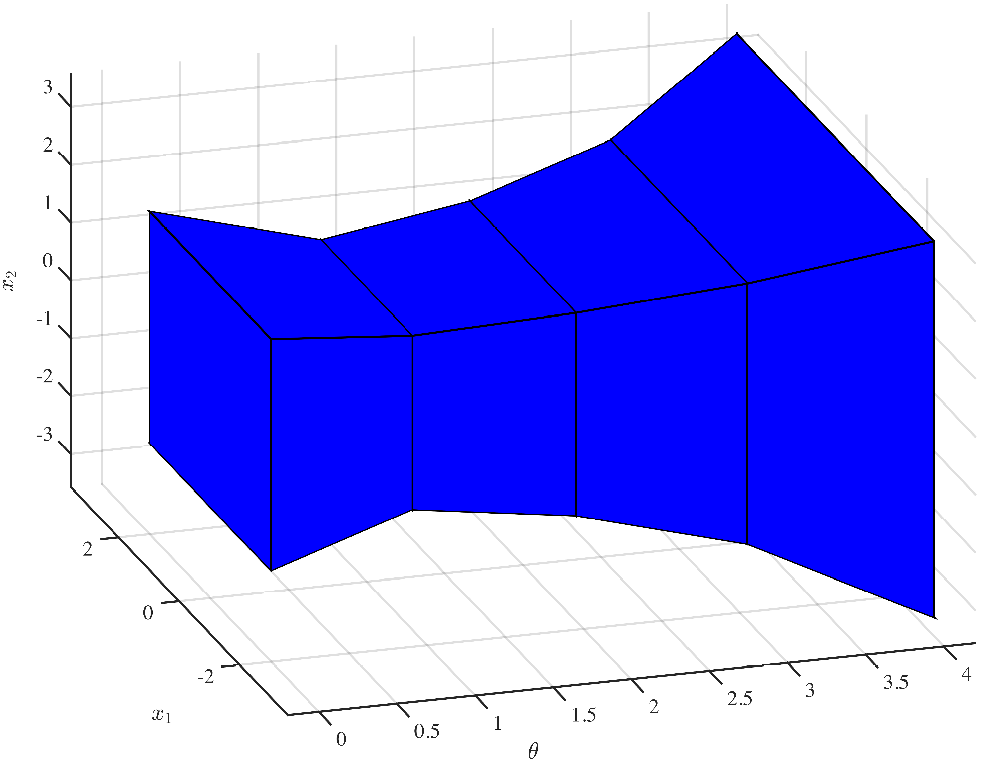
\includegraphics[width=.7\textwidth]{ParametricConvexSet}
\caption[A parametrically convex set.]{The piecewise affine parametric set $\mathcal X(\theta)$ 
defined by $\mathcal X(\theta)\mathrel{\mathop:}=\left\{x:\norm{x}_\infty\leq\max\{-\frac{1}{2}
\theta+2,\frac{1}{4}\theta+\frac{1}{5},\frac{1}{2}\theta+\frac{3}{4},\theta-\frac{3}{4}\}\right\}$ 
for $\theta\in[0,4]$. $\mathcal X(\theta)$ is parametrically convex in~$\theta$.}
\label{fig:parametrically:convex:set}
\end{figure}
%
Notice that Definition~\ref{def:parametric:convexity} does not require convexity of~$\mathcal W(p)$ for all
$p\in X$, we will however only treat maps~$\mathcal W$ for which $\mathcal W(p)$ is convex.
%
In order to compute maximal positive invariant sets for the considered system we need to generalise
the Pontryagin set difference (see e.g.~\cite{blanchini:2007}) to accommodate parametrically convex sets.
%
\begin{defi}[Parametric Pontryagin Difference]\label{def:parametric:pontryagin:difference}
	Let $S\subseteq X$ and let $\mathcal W:X\to\mathcal P(X)$ be a continuous point-to-set map such that
	$\mathcal W(p)$ is convex for all $p\in X$, then the \emph{parametric Pontryagin difference} 
	$S\ominus \mathcal W(S)$ is 
	\begin{equation}\label{eq:definition:parametric:pontryagin:difference}
		S\ominus \mathcal W(S) = \left\{x\in X: \{x\} \oplus \mathcal W(x)\subseteq S\right\},
	\end{equation}
	where $\mathcal W(S)$ denotes the image of $S$ under the map $\mathcal W$. 
\end{defi}
%
At first it may seem sensible to generalise the Pontryagin difference even further and define
%
\begin{equation}\label{eq:extended:parametric:pontryagin:difference}
\begin{split}
	S\ominus \mathcal W(R) &= \{x:\{x\}\oplus \mathcal W(r)\subseteq S\,\forall\, r\in R\}\\
	&=\{x:\{x\}\oplus\bigcup_{r\in R} \mathcal W(r)\subseteq S\}.
\end{split}
\end{equation}
%
However, since $\bigcup_{r\in R} \mathcal W(r)$ may or may not be convex, we can not make any useful
statements about $S\ominus \mathcal W(R)$. 
%
In the case that~$\mathcal W(p)$ is constant, i.e. $\bigcup_{p\in X}\mathcal W(p)=\mathcal W(p)=:C$,
we see that $S\ominus \mathcal W(S)=S\ominus C$ which is the Pontryagin difference for regular sets.
%
For the parametric Pontryagin difference of a convex set and a parametrically convex map we 
have the following result.
%
\begin{thm}\label{thm:convexity:of:pontryagin:difference}
  Let $S\subseteq X$ be a convex set and let $\mathcal W:X\rightarrow\mathcal P(X)$ be a parametrically convex point-to-set
  map such that $\mathcal W(p)$ is convex for all $p\in X$, then $S\ominus \mathcal W(S)$ is convex.
\end{thm}
%
\begin{proof}
To prove the convexity of $ Z :=  S\ominus \mathcal W( S)$ we pick any $z_1,z_2\in Z$, then
by definition of the parametric Pontryagin difference, we have
%
\begin{equation}
	\{z_i\} \oplus \mathcal W(z_i) \subseteq S,\; i=1,2.
\end{equation}
%
To see that $ Z$ is convex we show that line segments between
all possible $z_1$ and $z_2$ are subsets of $ Z$, i.e.~for all $\lambda \in [0,1]$,
\begin{equation}
\begin{aligned}
	\{ \lambda z_1 + (1-&\lambda)z_2
	\}\oplus \mathcal W\left( \lambda z_1 + (1-\lambda)z_2\right)\\
	\subseteq&\left\{ \lambda z_1 + (1-\lambda)z_2
	\right\}\oplus \lambda \mathcal W(z_1) \oplus (1-\lambda)
	\mathcal W(z_2)\\
	\subseteq &\lambda\underbrace{(\{z_1\}\oplus \mathcal W(z_1))}_{\subseteq S}\oplus
	(1-\lambda)\underbrace{(\{z_2\}\oplus \mathcal W(z_2))}_{\subseteq S}\\
	\subseteq& Z
\end{aligned}
\end{equation}
%
where the last inclusion follows from the convexity of $\mathcal S$.
\end{proof}
%
% Now consider a parametrically convex set of the form
% %
% \begin{equation}\label{eq:parametric:polyhedron}
% 	T(s)=\{t:Gt\leq H(s)\},
% \end{equation}
% %
% where each row of $H(s)$ is a convex function in $s\in S$, i.e. each element $H_i(s)$ of 
% $H(s)$ satisfies $H_i(\lambda s_1+(1-\lambda)s_2)\leq \lambda H_i(s_1)+(1-\lambda)H_i(s_2)$ 
% for all $\lambda\in[0,1]$ and $s_1, s_2\in S$. 
% %
% We will use sets for which $H(s)$ is piecewise affine in $s\in S$, i.e. sets
% for which $H_i(s) = \max_k\{f_k s + g_k\}$.
% %
% For sets of this type we have the following result.
% %
% \begin{thm}\label{thm:convex:parametric:set}
%   The point-to-set map $T(s)$ defined by~\eqref{eq:parametric:polyhedron} is parametrically 
%   convex for all $s\in S$ if $H(s)$ is elementwise convex in $s\in S\subseteq X \subset 
%   \mathbb R^n$.
% \end{thm}
% %
% \begin{proof}
% To show that $T(\lambda s_1 + (1-\lambda)s_2)\subseteq \lambda T(s_1) \oplus(1-\lambda)
% T(s_2)$ for all $\lambda \in [0,1]$ and $s_1, s_2\in S$ we note that
% %
% \begin{equation}
% \begin{aligned}
%   T&(\lambda s_1 + (1-\lambda)s_2)\\
%   =& \{t:\; G t \leq H(\lambda s_1 + (1-\lambda)s_2)\}\\
%   \subseteq& \{t:\;Gt\leq\lambda H(s_1)+(1-\lambda) H(s_2)\}\\
%   =&\{t:\;Gt\leq\lambda H(s_1)\}\oplus\{t:\;Gt\leq(1-\lambda)H(s_2)\}\\
%   =&\lambda T(s_1)\oplus(1-\lambda) T(s_2).
%   \end{aligned}
% \end{equation}
% %
% \end{proof} 
% %
% Notice that rays and vertices of $T(s)$ as defined in~\eqref{eq:parametric:polyhedron} will
% be linear combinations of $H_i(s)$, this implies that for piecewise affine $H(s)$ rays
% and vertices $t_k(s)$ will themselves be piecewise affine in $s\in S$, we will exploit
% this fact later on.
%
%
In the following we derive a property for piecewise affine parametric set-valued maps that will
allow convenient computation, namely that it is sufficient to check the number of vertices of 
instances $\mathcal W(p)$ on the boundaries of the parameter space to guarantee the parametric convexity.
%
The statement is summarised in Corollary~\ref{thm:p:convexity:PWA:set:constant:num:verts} in this section.
%
First we introduce the \emph{graph} of $\mathcal W$
%
\[
	\mathscr G(\mathcal W) = \{(p,x) \in\mathbb R^{d+n}: x\in\mathcal W(p)\},
\]
%
its \emph{interior}
%
\[
	\text{int}(\mathscr G(\mathcal W)) = \{(p,x) \in\mathbb R^{d+n}: \forall d\in\mathbb R^n\;\exists 
	\epsilon>0 : x+\epsilon d\in \mathcal W(p)\}
\]
%
and its \emph{boundary}
\[
	\partial \mathscr G(\mathcal W) = \mathscr G(\mathcal W)\setminus \textup{int}(\mathscr G(\mathcal W)).
\]
%
We define the \emph{extended normal cone} as
%
\[
	\mathcal N\mathcal W(p,x) = \{d\in\mathbb R^n: x+\epsilon d \not\in \mathcal W(p)\; \forall \epsilon>0\}
\]
for all $(p,x)\in\partial\mathscr G(\mathcal W)$.
%
\begin{rem}
%
Notice that we define the extended normal cone without an inner product. 
%
The way it is defined here, the conventional normal cone (e.g.~\cite{Boyd:04}) for a convex set $\mathcal C$
%
\[
	N_{\mathcal C}(x) = \{y: \langle y,x-z\rangle\geq0\;\forall z\in\mathcal C\}
\]
%
is be contained in the extended normal cone
%
\[
	\mathcal N_{\mathcal C}(x) = \{y:\exists\epsilon>0\;x+\epsilon y\not\in\mathcal C\}.
\]
%
Furthermore, we have that $\langle d, y\rangle\geq0$ for all $d\in\mathcal N_{\mathcal C}(x), y\in N_{\mathcal C}(x)$.
%
\end{rem}
%
\begin{rem}
%
Notice further that all definitions above are defined relatively for the \emph{set variable} $x$ rather than for graph
variable $(p,x)$.
%
\end{rem}
%
We state the central theorem to connect parametric convexity of a set valued map $\mathcal W$ with properties of its graph
$\mathscr G(\mathcal W)$.
%
\begin{thm}\label{thm:p:convexity:graph}
The map $\mathcal W$ is parametrically convex iff for all $(p_1,x_1),(p_2,x_2)\in\partial\mathscr G(\mathcal W)$
with $\mathcal N\mathcal W(p_1,x_1)\cap\mathcal N\mathcal W(p_2,x_2)\neq\emptyset$ and $p_1\neq p_2$ 
%
\begin{equation}\label{eq:graph:def:p:convexity}
\lambda (p_1,x_1) + (1-\lambda) (p_2,x_2) \not\in\textup{int} (\mathscr G(\mathcal W))
\end{equation}
%
holds for all $\lambda\in(0,1)$.
%
\end{thm}
%
\begin{proof}
%
Assume~\eqref{eq:graph:def:p:convexity} holds for $(p_1,x_1),(p_2,x_2)\in\partial\mathscr G(\mathcal W)$.
%
Then the Minkowski functional (see e.g.~\cite{Rudin:91}) yields $\mu(\mathcal W(\lambda p_1 + (1-\lambda)p_2),
\lambda x_1+(1-\lambda)x_2)\geq1$,
i.e. all interpolation points lie either on the boundary or outside the set $\mathcal W(\lambda p_1+(1-\lambda)p_2)$
therefore the set of all possible interpolation points 
%
\[
	\lambda \mathcal W(p_1)\oplus (1-\lambda)\mathcal W(p_2) = \{x:x=\lambda x_1 + (1-\lambda) x_2 \wedge x_1\in\mathcal 
	W(p_1) \wedge x_2\in\mathcal W(p_2)\}
\]
%
contains the set $\mathcal W(\lambda p_1 + (1-\lambda)p_2)$.
%
Now assume $\mathcal W$ is parametrically convex but~\eqref{eq:graph:def:p:convexity} is not satisfied for 
some $(p_1,x_1),(p_2,x_2)\in\partial\mathscr G(\mathcal W)$ with $\mathcal N\mathcal W(p_1,x_1)\cap\mathcal 
N\mathcal W(p_2,x_2)\neq\emptyset$, i.e. $\lambda x_1 + (1-\lambda)x_2\in\text{int}(\mathcal W(\lambda p_1 + 
(1-\lambda)p_2)$.
%
This implies that a full dimensional ball $B_\epsilon(x ) = \{y:\| 
x-y\|<\epsilon\}$
is contained in $\mathcal W(\lambda p_1 + (1-\lambda)p_2)$, i.e. $B_\epsilon(\lambda x_1 + (1-\lambda)x_2 )\subset
\mathcal W(\lambda p_1 + (1-\lambda)p_2)$ for some $\epsilon>0$.
%
Since $\mathcal N\mathcal W(p_1,x_1)\cap\mathcal N\mathcal W(p_2,x_2)\neq\emptyset$, there exist directions 
$d\in\mathcal N\mathcal W(p_1,x_1)\cap\mathcal N\mathcal W(p_2,x_2)$ which can not be represented as $d=\lambda d_1+
(1-\lambda)d_2$ with $x_1 + \epsilon d_1\in\mathcal W(p_1)$ and $x_2  + \epsilon d_2\in\mathcal W(p_2)$, however since $B_\epsilon$ is full dimensional
all directions exist, $x+\epsilon d\in\mathcal W(\lambda p_1 + (1-\lambda)p_2)$.
%
Hence, $\mathcal W$ can not be parametrically convex.
\end{proof}

\begin{rem}
Notice that condition~\eqref{eq:graph:def:p:convexity} is a non-convexity condition on the graph $\mathscr G(\mathcal W)$.
%
If $\mathscr G(\mathcal W)$ is strictly convex anywhere~\eqref{eq:graph:def:p:convexity} is violated and 
$\mathcal W$ can not be parametrically convex.
\end{rem}
%
\begin{rem}
%
Furthermore notice that the condition on the extended normal cones is only a restriction on the choice of 
$(p,x)$.
%
It is to avoid choices such that the entire line between $(p_1,x_1)$ and $(p_2,x_2)$ is contained in the interior
of the graph by convexity of $\mathcal W(p_i)$.
%
\end{rem}
%
\begin{figure}
\centering 
\begin{lpic}{pConvexSetsAbstract}
\lbl{74,16;$p$}
\lbl{52,20,90;$\mathcal W(p_2)$}
\lbl{10,20,90;$\mathcal W(p_1)$}
\lbl[bl]{17,35,45;$\mathcal N\mathcal W(p_1,x_1)$}
\lbl[bl]{58,37,45;$\mathcal N\mathcal W(p_2,x_2)$}
\lbl[bl]{62,17,45;$\textup{int}(\mathscr{G}(\mathcal W))$}
\lbl[l]{77,4;$\partial \mathscr{G}(\mathcal W)$}
\end{lpic}
\caption[Example p-convex set]{Illustration of the concepts for a scalar parametrically convex map in one-dimension.}
\end{figure}
%
\begin{cor}
%
Let $\mathcal W(p):=\{x\in\mathbb R^n: r(p,x)\leq0\}$ define a set-valued map with a continuous function 
$r: \mathbb R^d \times\mathbb R^n \rightarrow \mathbb R,(p,x)\mapsto r(p,x)$, then $\mathcal W$ is parametrically
convex iff the function $r$ is concave in $p\in\mathbb R^d$ and convex in $x\in\mathbb R^n$.
%
\end{cor}
%
\begin{proof}
The convexity in $x\in\mathbb R^n$ is required to satisfy the requirement that $\mathcal W(p)$ is convex
for all fixed values of $p\in\mathbb R^d$. 
%
Assume that for some region $\Omega\subset\mathbb R^d$ the function $r(\cdot,x)$ is non-concave (i.e. 
strictly convex), any convex subset $\mathcal C\subseteq\Omega$ will hence be such that $\mathscr 
G(\mathcal W)\vert_{\mathcal C}$ is a convex set.
%
In particular all lines between all $(p_1,x_1),(p_2,x_2)\in \partial\mathscr G(\mathcal W)\vert_{\mathcal C}$ will satisfy
$\lambda (p_1,x_1) + (1-\lambda) (p_2,x_2) \in\textup{int} (\mathscr G(\mathcal W))\vert_{\mathcal C}$ since
$\mathscr G(\mathcal W)\vert_{\mathcal C}$ is strictly convex in $p$.
%
This implies that $r(\cdot,x)$ can not be non-concave in any non-trivial set $\Omega\subseteq\mathbb R^d$ and still
be parametrically convex.
\end{proof}
%
\begin{cor}\label{thm:polytopic:set:not:p:convex}
The polytopic parametric set valued map $\mathcal W(p):=\{x: a_i x + b_i p\leq c_i \forall i\leq m\}$ is not parametrically convex for 
any non-trivial matrix $B$.
\end{cor}
%
\begin{proof}
The graph $\mathscr G(\mathcal W)$ is given by
%
\begin{equation*}
	\mathscr G(\mathcal W) = \{(p,x):a_i x + b_i p\leq c_i \forall i\leq m\}
\end{equation*}
%
and hence is a convex set and violates Theorem~\ref{thm:p:convexity:graph}.
\end{proof}
%
We now can prove the following central corollary.
%
\begin{cor}\label{thm:p:convexity:PWA:set:constant:num:verts}
The piecewise affine polytopic parametric set valued map 
%
\begin{equation}\label{eq:definition:PWA:polytopic:set:general}
	\mathcal W(p) := \left\{x: a_i x \leq \max_{k\leq l}\{b_{i,k} + C_{i,k}p\},i\leq m\right\}
\end{equation}
%
is parametrically convex iff the number of vertices $v_i(p)$ and rays $u_i(p)$ is constant.
\end{cor}
%
\begin{proof}
For clarity this proof is divided in 3 parts:
\begin{enumerate}
\item Notice that $h_i(p) = \max_{k\leq l} \{b_{i,k} + C_{i,k}p\}$ is a multi-parametric linear program (mpLP),
its solution is a piecewise affine function $h_i(p) = b_{i,k^\ast_i} + C_{i,k^\ast_i}p$ where $k^\ast_i(p)$ is constant
inside a polytopic complex, see e.g.~\cite{spjotvold:2005}.
%
That means that there exists a finite partitioning $\mathbb R^d = \bigcup_{i\leq t} \mathcal P_i$ with convex polyhedra 
$\mathcal P_i$ such that ${\bf{k}}^\ast\vert_{\mathcal P_i} = (k_1^\ast,\dots,k_m^\ast) = const$.
%
A standard degeneracy assumption is that in neighbouring partitions ${\bf{k}}^\ast\vert_{\mathcal P_i}$ and 
${\bf{k}}^\ast\vert_{\mathcal P_j}$ differ in exactly one element.
%
This partitioning implies that the graph $\mathscr G(\mathcal W)$ is given as a finite union of polyhedra
%
\begin{equation*}
	\mathscr G(\mathcal W) = \bigcup_{j\leq t} \left\{x: a_i x \leq b_{i,k_i^\ast} + C_{i,k_i^\ast}p,i\leq m
	\right\}\bigr\vert_{\mathcal P_j}
\end{equation*}
%
But this implies that if the number of vertices or rays changes in any partition $\mathcal P_i$ then $\mathscr
G(\mathcal W)\vert_{\mathcal P_i}$ is a strictly convex polytope and theorem~\ref{thm:polytopic:set:not:p:convex} applies.
%
\item Our attention hence is concentrated to the boundaries of the partitions $\mathcal P_i$.
%
These are the points $\mathcal P_i \cap \mathcal P_j$ where some mpLP changes its solution, i.e. 
$b_{i,k_{i_1}^\ast} + C_{i,k_{i_1}^\ast} p = b_{i,k_{i_2}^\ast} + C_{i,k_{i_2}^\ast} p$.
%
Notice that a vertex $v_i(p)$ is given by \emph{active} and \emph{inactive} inequalities, i.e. $\mathcal A_i(p)$ and
$\mathcal I_i(p) = \{1,\dots,m\}\setminus\mathcal A_i(p)$ respectively.
%
\begin{equation*}\begin{split}
	a_j v_i(p) &= b_{j,k_j^\ast} + C_{j,k_j^\ast} p \quad\forall j\in\mathcal A_i(p)\\
	a_j v_i(p) &< b_{j,k_j^\ast} + C_{j,k_j^\ast} p \quad\forall j\in\mathcal I_i(p)
\end{split}\end{equation*}
%
In order for the number of vertices to change, there must be a hyperplane $fp=g$, such that the number of vertices for $fp<g$ is 
$N$ and for $fp>g$ is at least $N+1$.
%
It follows from the previous discussion that $\{p:fp=g\} = \textup{aff}\{\mathcal P_i\cap\mathcal P_j\}$ for some $i\neq j$.
%
For vertices $v_i(p)$ and $v_j(p)$ to merge the index sets $\mathcal A_i(p)$ and $\mathcal A_j(p)$ have to differ in only one 
element, i.e. $\mathcal A_i(p) = \mathcal J\cup \{s\}$ and $\mathcal A_j(p) = \mathcal J\cup\{u\}$ for $fp>g$.
%
Furthermore, for $p$ with $fp\leq g$ we have $v_i(p)=v_j(p)$, this implies $\mathcal A_i(p) = \mathcal A_j(p)$.
%
Since only one alteration of the active index set is considered (due to generic assumptions), the active set $\mathcal A_i(p) = \mathcal A_j(p)
= \mathcal J \cup \{s,u\}$.
%
Hence on the hyperplane $fp=g$ both, the maximising index ${\bf{k}}^\ast(p)$ and the active index sets $\mathcal A_i(p)$ 
and $\mathcal A_j(p)$ change, which is degenerate.
%
\item In order for the degenerate graph $\mathscr G(W)$ to be parametrically convex the overdetermined vertex $v_i(p)=v_j(p)$
have to be identical, in particular their dependence on $p$ has to be identical.
%
This can be expressed with the implicit function theorem:
%
\begin{equation*}\begin{split}
	\frac{d}{dp}\left(	A_{\mathcal J\cup \{s\}} v_i(p) - b_{\mathcal J\cup \{s\}} - C_{\mathcal J\cup \{s\},{\bf{k}}^\ast} p\right) &= 0\\
	\frac{d}{dp}\left(	A_{\mathcal J\cup \{u\}} v_i(p) - b_{\mathcal J\cup \{u\}} - C_{\mathcal J\cup \{u\},{\bf{k}}^\ast} p\right) &= 0
\end{split}\end{equation*}
%
which leads to 
%
\begin{equation*}\begin{split}
	A_{\mathcal J\cup \{s\}} \frac{dv_i}{dp} &= C_{\mathcal J\cup \{s\},{\bf{k}}^\ast}\\
	A_{\mathcal J\cup \{u\}} \frac{dv_i}{dp} &= C_{\mathcal J\cup \{u\},{\bf{k}}^\ast}
\end{split}\end{equation*}
%
since we can assume that the inequalities are non-redundant for some right hand side, we obtain that 
%
\begin{equation}\label{eq:derivative:condition:on:index:sets}
	\frac{dv_i}{dp} = A_{\mathcal J\cup \{s\}}^{-1}C_{\mathcal J\cup \{s\},{\bf{k}}^\ast} = 
	A_{\mathcal J\cup \{u\}}^{-1}C_{\mathcal J\cup \{u\},{\bf{k}}^\ast}
\end{equation}
%
has to hold for the degenerate graph to remain parametrically convex.
%
Notice that~\eqref{eq:derivative:condition:on:index:sets} is again a degenerate condition, since arbitrarily small perturbations
will produce different behaviour.
\end{enumerate}
\end{proof}
%
\begin{rem}
Corollary~\ref{thm:p:convexity:PWA:set:constant:num:verts} is essential for numerical examples, as it can be reformulated to:
%
The set valued map defined by~\eqref{eq:definition:PWA:polytopic:set:general} is parametrically convex iff it has a constant 
number of vertices throughout the parameter space~$X$.
%
\\[1em]
%
Since the map is continuous it is sufficient to verify this at the vertices of the parameter space.
%
\end{rem}
%
To illustrate the effects of perturbations to a degenerate piecewise affine map, consider the following low dimensional 
examples:
%
\begin{quote}
Let $\mathcal W_i(p)$ be defined by
%
\begin{equation*}\begin{split}
	\mathcal W_1(p) = \left\{x : \left(\begin{array}{cc}
	1&1\\
	-1&1\\
	0&1\\
	0&-1 
	\end{array}\right)x \leq \left(\begin{array}{c}
	\max\{1+p,\frac{1}{2}+2p\} \\
	\max\{1+p,\frac{1}{2}+2p\} \\
	\frac{1}{2}+2p \\
	1
	\end{array}\right)
	\right\}\\
%
	\mathcal W_2(p) = \left\{x : \left(\begin{array}{cc}
	1&1\\
	-1&1\\
	0&1\\
	0&-1 
	\end{array}\right)x \leq \left(\begin{array}{c}
	\max\{1+p,\frac{1}{2}+(2+\epsilon)p\} \\
	\max\{1+p,\frac{1}{2}+2p\} \\
	\frac{1}{2}+2p \\
	1
	\end{array}\right)
	\right\}\\
%
	\mathcal W_3(p) = \left\{x : \left(\begin{array}{cc}
	1&1\\
	-1&1\\
	0&1\\
	0&-1 
	\end{array}\right)x \leq \left(\begin{array}{c}
	\max\{1+p,\frac{1}{2}+\epsilon+2p\} \\
	\max\{1+p,\frac{1}{2}+2p\} \\
	\frac{1}{2}+2p \\
	1
	\end{array}\right)
	\right\}
	\end{split}
\end{equation*}
%
%
\begin{figure}
\begin{center}
\subfigure[$\mathcal W_1(p)$]{\includegraphics[width=.45\textwidth]{pConvDegenerateSet}}
\subfigure[$\mathcal W_2(p)$]{\includegraphics[width=.45\textwidth]{pConvPertInLinTerm}}\\
\subfigure[$\mathcal W_3(p)$]{\includegraphics[width=.45\textwidth]{pConvPertInConstantTerm}}
\end{center}
\caption[Degenerate PWA p-convex sets]{For $\mathcal W_1(p)$ the right hand side was chosen in order 
to satisfy~\eqref{eq:derivative:condition:on:index:sets} 
and for the graph to be degenerate. For both $\mathcal W_{2,3}(p)$ there is no drop in number of vertices for different 
$p\in[-1,\infty),\epsilon=10^{-1}$.}
\label{fig:degenerate:PWA:set:and:comparison}
\end{figure}
%
See figure~\ref{fig:degenerate:PWA:set:and:comparison} for an illustration.
\end{quote}
%
The number of vertices and rays can be large for complex sets~$\mathcal W(p)$, therefore it can be 
useful to analyse the irreducibility of the given halfspace description. This alternative is presented in 
appendix~\ref{app:irreducibility:PWA:sets}.
%
%
%
%
\section{Example}\label{sec:example:linearisation:error:as:state:dependent:constraint}
In this section we derive a disturbance set that is of the form~\eqref{eq:derivative:condition:on:index:sets}
with a piecewise affine right hand side~$H(s)$. 
%
Consider a discrete time nonlinear system of the form
%
\begin{equation}
	x^+ = f(x,u)
\end{equation}
%
with $x_e=f(x_e,u_e)$ as an equilibrium point. 
%
Close to the equilibrium point the dynamics can be approximated by ${\tilde x}^+ = A \tilde x 
+ B\tilde u$ with $\tilde x = x-x_e$ and $\tilde u = u - u_e$ and the linearisation matrices
$A = \frac{\partial f}{\partial x}\vert_{(x_e,u_e)}$ and $B = \frac{\partial f}{\partial u}
\vert_{(x_e,u_e)}$.
%
We want to describe the dynamics of the nonlinear system with those of its linearisation considering
an additive disturbance. 
%
I.e. we want that for all $x\in X_c$ and $u\in U_c$ there exists a realisation 
$v\in V(x,u)$ such that the identity $f(x,u)=Ax + B u + v$ holds. 
%
In order to derive a parametrised set $V(x,u)$ such that the desired identity holds we use
the mean value theorem (see e.g.~\cite{Apostol:1974}):
%
\begin{thm}[Mean Value Theorem]\label{thm:mean:value:theorem}
Let $g : \mathcal X \rightarrow\mathbb R^m$ be continuously
differentiable, $\mathcal X\subset\mathbb R^n$ be open,
and $x \in\mathcal X$, $h \in\mathbb R^n$ be such that 
$x + th \in\mathcal X$ for all $t\in [0 ,1]$. Then
\begin{equation}
	g(x+h) = g(x) + \left(\int_0^1 \frac{\partial g}{\partial x}(x+th)dt\right)\cdot h.
\end{equation}
\end{thm}
%
We can use this to state
%
\begin{equation}
\begin{split}
	f(x_e+x,u_e+u)-A(x_e+x)-B(u_e+u) = \underbrace{f(x_e,u_e) - A x_e - B u_e}_{=0} \\
	+ \int_0^1\left(\frac{\partial f}{\partial x}(x_e+tx,u_e+tu) \cdot x + 
	\frac{\partial f}{\partial u}(x_e+tx,u_e+tu) \cdot u \right) dt -Ax-Bu\\
	= \underbrace{\left(\int_0^1 \frac{\partial f}{\partial x}(x_e+tx,u_e+tu) dt - A\right)}_{H^x} x + 
	\underbrace{\left(\int_0^1 \frac{\partial f}{\partial u}(x_e+tx,u_e+tu) - B \right)}_{H^u} u.
\end{split}
\end{equation}
%
This means that for any given $(x,u)\in X\times U$ we can compute an additive disturbance $v=H^x x + H^u u$
such that $f(x_e+x,u_e+u)-Ax-Bu = v$.
%
Assume we had all possible $H^x$ and $H^u$ for all $(x,u)\in X\times U$ given, clearly then 
$\min\{H^x x + H^u u\} \leq f(x_e+x,u_e+u)-Ax-Bu \leq \max\{H^x x + H^u u\}$ holds true.
%
For general nonlinear systems there is no way to obtain an analytic solution for $H^x$ and $H^u$,
so instead $K$ samples of $X\times U$ have to be used to obtain a description of 
the disturbance set
%
\begin{equation}\label{eq:derivation:of:PWA:disturbance:set}
\begin{split}
	V^K(x,u) &= \left\{v: \min_{k\leq K}\{H^x_k x + H^u_k u\} \leq v \leq \max_{k\leq K}\{H^x_k x + H^u_k u\} \right\}\\
	&= \left\{v: v \leq \max_{k\leq K}\{H^x_k x + H^u_k u\} \wedge -v \leq \max_{k\leq K}\{-H^x_k x - H^u_k u\} \right\}
\end{split}
\end{equation}
%
Notice that sampling the set $\gimel(x,u) = \left\{v : \min\{H^x x + H^u u\} \leq v \leq \max\{H^x x + H^u u\}\right\}$ 
leads to an inner approximation which is convexified by taking its convex hull.
%
The set $V^K(x,u)$ as defined in~\eqref{eq:derivation:of:PWA:disturbance:set} is of the
type~\eqref{eq:derivative:condition:on:index:sets} with a piecewise linear right hand side. We may
want to add a constant term to accommodate model uncertainties.
%
%
%
%
\section{Maximal Positive Robust Invariant Sets}\label{sec:parametrised:MRPI:set}
In this section we present a way to calculate maximal robust positive invariant sets for
linear discrete time systems under the influence of additive perturbation.
%
We assume the perturbation to be constrained in sets which are piecewise affine in
the state, i.e.
%
\begin{equation}\label{eq:definition:PWA:uncertainty}
v\in \mathcal V(x) = \left\{v: Gv\leq\max_k\{H_k^x x + h_k\}\right\}.
\end{equation}
%
The definition of the maximal robust positive invariant set in this scenario is given as
the largest set satisfying
%
\begin{equation}\label{eq:MRPI:state:dependent:disturbance}
	\mathcal X^\infty = \left\{x: \Psi x + v \in\mathcal X^\infty\,\forall\, v\in\mathcal V(x)\right\},
\end{equation}
%
largest in the sense that it includes all smaller ones.
%
The implicit definition of~\eqref{eq:MRPI:state:dependent:disturbance} suggests a recursive 
computation of $\mathcal X^\infty$.
%
We assume system dependent state constraints $\mathscr X\subseteq\mathbb R^n$ are given,
we furthermore assume that $\mathscr X$ is polyhedral and contained in a band.
%
\begin{defi}[Band Property]
We say that a set $X\subseteq\mathbb R^d$ possesses the band property if there exists a 
matrix~$\Gamma\in\mathbb R^{p\times d}$ such that $X\subseteq B = \{x:\Gamma x\leq {\bf{1}}\wedge
-\Gamma x\leq{\bf{1}}\}.$
\end{defi}
%
That is, we assume that $\mathscr X= \{x:\Lambda_i x \leq \lambda_i \forall\, i\leq m\}\subseteq\{x:\Gamma x\leq{\bf{1}}\wedge
-\Gamma x\leq{\bf{1}}\}=:\mathscr B$.
%
In the following we discuss how to apply the principle of the Kolmanovsky and Gilbert 
algorithm\footnote{The concept was first introduced for 
unperturbed systems in 1991 by Gilbert and Tan~\cite{Gilbert:1991}, therefore all its derivatives 
are also referred to as the \emph{Gilbert and Tan algorithms}.} 
presented in~\cite{Kolmanovsky:1995}.
%
The algorithm is a recursive iteration: Starting from $\mathscr X$ we 'cut off' all such stated 
for which the successor state would violate~\eqref{eq:MRPI:state:dependent:disturbance}, i.e.
in the $n^\text{th}$~iteration we introduce constraints which enforce that the trajectories
of all points in the set would remain in the set for $n$~time steps.
%
This means that in the first iteration we enforce that for all points in the iterate the 
successor state is contained in the initial set $x^+\in X_0 = \mathscr X$:
%
\begin{equation}\label{eq:PWA:disturbance:first:iterate}
\begin{split}
	X_1 &= \{x: \Psi x + v\in X_0 \forall v\in\mathcal V(x)\}\\
	&=\{x:\Lambda_i(\Psi x +v)\leq \lambda_i \forall\,i\leq m_0\}\\
	&=\left\{x:\Lambda_i\Psi x + 
	\underbrace{\left\{\begin{array}{rl}\max& \Lambda_i v\\ 
	\text{s.t.}& v\in\mathcal V(x)
	\end{array}\right\}}_{\gamma_{1,i}^\ast(x)} \leq \lambda_i \forall\,i\leq m_0\right\}
\end{split}
\end{equation}
This requires the solution $m_0$ multi-parametric linear programs\footnote{Multi-parametric 
linear programs have been introduced as optimisation problems
in the late 1958 by~\cite{Courtillot:1958}. Various ways to solve mpLPs have been proposed.}
(mpLPs) in order to obtain~$v_{1,i}^\ast(x)$.
%
However, the solution of multi-parametric linear programs will be given by vertices 
of the constraint set, i.e. $\gamma_{1,i}^\ast(x)=\Lambda_i v_{k^\ast}(x)$ where $v_{k^\ast}(x)$
is the optimising vertex.
%
Recall that since $\mathcal V(x)$ is piecewise affine in $x$ its vertices will also be piecewise 
affine in $x$, i.e. there exists a representation $v_k(x)=\max_{l\leq K_k}\{W_l^k x + w_l^k\}$.
%
Notice that we do not need to solve all mpLP in order to compute $X_1$, adding all available
$W_l,w_l$ produces the desired set without solving $m_0$ mpLP:
%
\begin{equation}\label{eq:derivation:of:row:reduction:instead:of:mpLP}
\begin{split}
	X_1 &= \{x: \Lambda_i\Psi x + \gamma_{1,i}^\ast(x)\leq\lambda_i \,\forall i\leq m_0 \}\\
	&= \left\{x: \Lambda_i\Psi x + \max_l\{\Lambda_i (W_l^{k^\ast} x + w_l^{k^\ast}) \} \leq \lambda_i\, 
	\forall i\leq m_0 \right\} \\
	&= \left\{x: (\Lambda_i\Psi + \Lambda_i W_l^{k^\ast}) x \leq \lambda_i-\Lambda_i w_l^{k^\ast}\,
	\forall i\leq m_0, l\leq K_k  \right\} \\
	&= \left\{x: (\Lambda_i\Psi + \Lambda_i W_l^k) x \leq \lambda_i - \Lambda_i w_l^k\,
	\forall i\leq m_0, l\leq K_k, k\leq \kappa \right\}.
\end{split}
\end{equation}
%
The equalities~\eqref{eq:derivation:of:row:reduction:instead:of:mpLP} hold since only the 
inequalities which define~$\gamma_{1,i}^\ast(x)$ will define the set~$X_1$, i.e. we avoid
solving mpLP by introducing redundant inequalities, instead of $m_0$ supporting hyperplanes
we describe the set by $m_1 = m_0\cdot \kappa\cdot \prod_{k\leq \kappa} K_k$ hyperplanes with
a large number of them being redundant, here~$\kappa$ denotes maximal the number of vertices 
of~$\mathcal V(x),\,x\in\mathscr X$.
%
This seems to be a poor trade off, however, we can use inequality reduction algorithms at any
point of the iteration and reduce the number of hyperplanes~$m_1$ in the representation of~$X_1$.

The next set iterate~$X_2$ is then defined by
%
\begin{equation}
	\begin{split}
	X_2 &= \left\{x: \Psi (\Psi x + v) + \tilde v\in X_0\,\forall v,\tilde v\in\mathcal V(x) \right\}\\
	&= \{x\in X_1 : \Psi x + v \in X_1\,\forall v\in\mathcal V(x)\}\\
	&= X_1 \cap \{x: \Psi x + v \in X_1\,\forall v\in\mathcal V(x)\},
	\end{split}
\end{equation}
%
so that successive set iterates can be defined recursively.
%
The general iterate is given by:
%
\begin{equation}\label{eq:general:MRPI:iteration}
	X_{k+1} = X_k \cap \{x:\Psi x + v\in X_k\, \forall v\in\mathcal V(x)\}
\end{equation}
%
It is obvious that by its definition $X_{k+1}\subseteq X_k$, once $X_k\subseteq X_{k+1}$ holds
the iteration~\eqref{eq:general:MRPI:iteration} terminates.
%
$X_k\subseteq X_{k+1}$ implies that all $x\in X_k$ also satisfy $x\in X_{k+1}$, however
$X_{k+1}$ is defined as points to which the successor state is contained in $X_k$, therefore
$X_{k+1} = \mathcal X^\infty$. 

In the remainder of this section we will prove that the described algorithm terminates 
in a finite number of iterations.
%
Notice that the set iterates defined by~\eqref{eq:general:MRPI:iteration} can be formally
be defined by
%
\begin{equation}
	X_{k+1} = X_k \cap \{x: \Lambda_i\Psi^k x + \sum_{l=1}^{k-1} \gamma_{l,i}^\ast(x)\leq\lambda_i\,
	\forall i\leq m_0\},
\end{equation}
%
where
%
\begin{equation}\begin{split}
	\gamma_{l,i}^\ast(x) &= \max_j \Lambda_i\Psi^{l-1} v_j(x) \\
	&= \begin{array}{rl} \max_v &\Lambda_i\Psi^{l-1} v\\
		\text{s.t.} & v\in\mathcal V(x)\end{array} \\
	&= \begin{array}{rl} \max_{\tilde v} &\Lambda_i \tilde v\\
		\text{s.t.} & \tilde v\in \Psi^{l-1}\mathcal V(x) \end{array}.
\end{split}\end{equation}
%
So that~\eqref{eq:general:MRPI:iteration} becomes
%
\begin{align}
	X_{k+1} &= X_k \cap \left( \Psi^{-k-1} X_0\, \underset{1\leq i\leq k}{\bigominus} 
	\Psi^{i-1}\mathcal V(X_k) \right)\nonumber \\
	&=\bigcap_{l\leq k+1}\left(\Psi^{-l} X_0 \underset{1\leq i\leq l-1}{\bigominus} 
	\Psi^{i}\mathcal V(X_{l-1}) \right). \label{eq:MRPI:recursion:closed:form}
\end{align}
%
The structure of~\eqref{eq:MRPI:recursion:closed:form} is of central importance for the proof
of finite determinability of~$\mathcal X^\infty$.
%
The first statement we can prove is the following:
%
\begin{thm}\label{thm:band:implies:compactness}
Let the system constraints be contained in a band~$\mathscr X\subseteq \mathscr B 
=\{x: \Gamma x\leq{\bf{1}}\wedge -\Gamma x\leq{\bf{1}}\}$, let $0\in\mathcal V(x)$ for all $x\in\mathscr X$ 
and let the pair $(\Psi,\Gamma)$ be observable, then there exists a natural number $N\leq n$ such 
that~$X_N$ is compact.
\end{thm}
%
\begin{proof}
First recall the fact that $\mathcal A\ominus \mathcal B\subseteq\mathcal A$ if $0\in\mathcal B$,
see e.g.~\cite{blanchini:2007}, this fact extends to the parametric Pontryagin difference.
%
Therefore we have
%
\begin{equation}
	X_k= \bigcap_{l\leq k}\left(\Psi^{-l} X_0 \underset{1\leq i\leq l-1}{\bigominus} 
	\Psi^{i}\mathcal V(X_{l-1}) \right) \subseteq \bigcap_{l\leq k} \Psi^{-l} X_0
	= \bigcap_{l\leq k} \Psi^{-l}\mathscr X \subseteq \bigcap_{l\leq k} \Psi^{-l} \mathscr B.
\end{equation}
%
Note that observability of $(\Psi,\Gamma)$ is equivalent to the observability matrix
\[
	\Omega_o = \left(\begin{array}{c}
	\Gamma \\ \Gamma \Psi \\ \vdots \\ \Gamma \Psi^{n-1}
	\end{array}\right)
\]
%
has full rank.
%
This is equivalent to the null space of $\Omega_o$ being trivial, i.e.~$\ker\Omega_o=\{0\}$,
which implies that~$\{x: \Omega_o x \leq {\bf{1}} \wedge -\Omega_o x \leq {\bf{1}}\}$ is bounded.
%
Note further that
\begin{equation}
	X_n \subseteq \bigcap_{k\leq n} \Psi^{-k}\mathscr B = \left\{x:\underset{k\leq n}{\bigwedge} 
	\pm \Gamma\Psi^{k}x\leq{\bf{1}} \right\} =\{x: \Omega_o x \leq {\bf{1}}\wedge -\Omega_o x\leq{\bf{1}} \}.
\end{equation}
%
Therefore we conclude that $X_n$ is contained in a compact set, hence is itself bounded.
%
The case that~$N<n$ is possible for matrices $\Gamma$ with $\text{rank}(\Gamma)>1$.
\end{proof}
%
In the following we prepare to prove the statement:
%
\begin{thm}[\footnote{
	The earliest proof of finite determinability of the proposed algorithm was published 
	in~\cite[Theorem 4.2]{Kolmanovsky:1995}, the assumptions made for Lemma~\ref{thm:band:implies:compactness}
	and~\ref{thm:finite:terminability:MRPI:algorithm} coincide for the case of constant disturbance sets.
	%
	The formulation chosen here is more explicit than the one stated in~\cite{Kolmanovsky:1995}, since
	all conditions are on data available before initialising the algorithm.
	}]
\label{thm:finite:terminability:MRPI:algorithm}
Let the assumptions for Lemma~\ref{thm:band:implies:compactness} hold, let furthermore
$x^+=\Psi x$ be asymptotically stable, $\mathcal V(x)$ be bounded for all $x\in\mathscr X$ and let the Maximal Robust 
Positive Invariant Set contain an open ball, then iteration~\eqref{eq:general:MRPI:iteration} with~$X_0=\mathscr X$ 
terminates in a finite number of number of steps.
\end{thm}
\\[1em]
First we define the decay rate of a linear system.
%
\begin{defi}[Decay Rate]
For the linear discrete time system~$x[k+1] = \Psi[k] x[k]$ the \emph{decay rate} is given as the smallest value~$\lambda$ 
such that~$\lim_{k\rightarrow\infty}\lambda^{-k}\norm{x[k]}=0$
%
\footnote{Usually the decay rate is defined for continuous time systems $\dot x = A(t)x$ as the largest~$\alpha$ 
such that~$\lim_{t\rightarrow\infty}e^{\alpha t}\norm{x(t)}=0$ for all initial values $x_0$, see e.g.~\cite{Luenberger:1979}.
%
The reason to define $\lambda$ as the decay rate rather than $\lambda^{-1}$ is straight forward: 
%
The norm along a trajectory decays no slower than $\lambda^k\norm{x_0}$ which analogue to the continuous 
time~$e^{-\alpha t}\norm{x_0}$.}.
\end{defi}
%
Using a Lyapunov function~$V(x)>0$ for the system we can derive an upper bound on $\lambda$:
%
If $V[k+1]-V[k]\leq-\delta V[k]$ holds for all trajectories $x[k]$ (with $V[k] = V(x[k])$), then clearly the 
decay rate is bounded from above by $1-\delta$ since $V[k]\leq(1-\delta)^k V[0]$.
%
Assuming that the system is asymptotically stable we have that $V[k+1]>0$ and $V[k+1]-V[k]<0$, therefore we have~$0<1-\delta<1$
for all admissible choices of $V(x)$.
%
Since we are interested in linear systems only, we consider quadratic Lyapunov functions $V(x) = x^TPx$ with a positive
definite $P>0$, therefore we have that $\underline\sigma(P)^2\norm{x}_2^2\leq V(x)\leq \bar\sigma(P)^2\norm{x}_2^2$, 
where $\underline\sigma(P),\bar\sigma(P)$ denote the smallest and the largest singular values of $P$ respectively.
%
Together with $V(x+y)\leq V(x)+V(y)$ and $V(cx)=c^2 V(x)$ this means that~$\sqrt{V(x)}$ is a norm itself.
%
With this we can prove the statement:
%
\begin{thm}
Let $\Psi$ be non-singular and asymptotically stable and let $\rho(\Psi)$ denote its spectral radius, i.e. 
there exists at least one eigenvalue $\gamma$ and an eigenvector $v$ such that $\Psi v = \gamma v$ 
with $\abs{\gamma}=\rho(\Psi)$, then the bound $\rho(\Psi)^2\leq1-\delta$ is tight and is attained 
for $P=\Psi^T\Psi$.
\end{thm}
%
\begin{proof}
Using the test vector $\tilde\xi=\frac{v}{\norm{v}_P}$ we obtain $\gamma^\ast\tilde\xi^H P\tilde \xi\gamma
\leq(1-\rho)\tilde\xi^H P\tilde\xi$ but $\gamma^\ast\gamma = \abs{\gamma}^2 = \rho(\Psi)^2$.
%
The symmetric matrix $P = \Psi^T\Psi$ is positive definite for any invertible $\Psi$ and hence $\xi^T P\xi$ 
defines the square of a norm and using the same test vector we obtain $1-\delta=\rho(\Psi)^2$.
%
\end{proof}
%
The value of $1-\delta$ i.e. $\rho(\Psi)^2$ is also referred to as \emph{stability degree}, see e.g.~\cite{Boyd:94}.
%
In the sequel we abbreviate the spectral radius of $\Psi$ by $\rho$.
%
Notice that we can not prove that $\lambda=\rho^2$ since the norm in the definition of $\lambda$ is 
undefined and might be non-quadratic.

We use this result to bound the rate of convergence of $P$-ellipsoids $\mathcal E_P(r) = \{x:x^TPx\leq r^2\}$, i.e. 
the level set $V(x)\leq r^2$.
%
With the previous results $V(\Psi x)\leq \rho^2 V(x)$, which works analogously on the inverse 
$\rho^{-2}V(x)\leq V(\Psi^{-1} x)$, we have 
%
\begin{equation}\begin{split}
	\Psi\mathcal E_P(r) &= \{y=\Psi x:x^TPx\leq r^2\}\\
	&=\{x: \underbrace{(\Psi^{-1}x)^TP(\Psi^{-1}x)}_{\geq\rho^{-2} x^TPx}\leq r^2\}\\
	&\subseteq\{x: x^TPx\leq \rho^2 r^2\} = \mathcal E_P(\rho r)
\end{split}
\end{equation}
%
Recursively, we have 
%
\begin{equation}\label{eq:containment:Psik:subset:rhok}
	\Psi^k\mathcal E_P(r)\subseteq \mathcal E_P(\rho^k r)
\end{equation}
%
for the inverse $\Psi^{-1}$ we have $\Psi^{-1}\mathcal E_P(r)\supseteq\mathcal E_P(\rho^{-1}r)$ and 
$\Psi^{-k}\mathcal E_P(r)\supseteq\mathcal E_P(\rho^{-k}r)$.

To prove Lemma~\ref{thm:finite:terminability:MRPI:algorithm}, we first derive containment conditions of 
sets that are defined as level sets of norm:
%
Let the set $\mathscr F(r) := \{x:\norm{x}\leq r\}$ be the norm-ball of radius $r$, then the following statement holds 
for any norm~$\norm{\cdot}$.
% 
\begin{thm}\label{thm:inclusions:norm:balls:sum:difference}
The following two inclusions hold:
\begin{enumerate}
\item 
%
The norm ball of radius $r_1+r_2$ is contained in $\mathscr F(r_1)\oplus \mathscr F(r_2)$, i.e. 
%
\begin{equation}
	\mathscr F(r_1 + r_2)\subseteq \mathscr F(r_1)\oplus \mathscr F(r_2).
\end{equation}
%
\item
%
The ball of radius $r_1-r_2$ is contained in $\mathscr F(r_1)\ominus \mathcal F(r_2)$, i.e.
%
\begin{equation}
	\mathscr F(r_1-r_2)\subseteq \mathscr F(r_1)\ominus \mathscr F(r_2).
\end{equation}
\end{enumerate}
\end{thm}
%
\begin{proof}
%
Both statements follow from the triangle inequality.
%
For the first statement observe that $\norm{x+y}\leq r_1+r_2$ implies that $\norm{x}+\norm{y}\leq r_1+r_2$ which is equivalent to $\norm{x}\leq r_1\wedge\norm{y}\leq r_2$ which is the definition of $\mathscr F(r_1)\oplus \mathcal F(r_2)$.
%
The second statement follows since the Pontryagin difference is defined using the Minkowski sum:
%
If $\norm{z}\leq r_1 -r_2$ then $\norm{z+y}\leq\norm{z}+\norm{y}\leq r_1-r_2+r_2$.
\end{proof}
%
\begin{proof}[Proof of Lemma~\ref{thm:finite:terminability:MRPI:algorithm}]
Using~\eqref{eq:general:MRPI:iteration} we can easily see that if for some $k>0$
the set iterate $X_k$ is empty, we have $X_k=\mathcal X^\infty = \emptyset$,
in this trivial case we can easily see that the algorithm terminates after $k$ iterations.
%
In this case the assumption that there exists an open ball in the MRPI set is violated.
%
For the remainder of this proof we assume that all set iterates are non-empty.

We define the non-compact set iterates $\mathscr D_k = \Psi^{-1}\mathscr D_{k-1}\ominus \Psi^{-1}\mathcal V(\Psi^{-1}
\mathscr D_{k-1})$ starting from $\mathscr D_0 = X_0$, that is $\Psi\mathscr D_k\oplus \mathcal V(\mathscr D_k)
\subseteq\mathscr D_{k-1}$.
%
So that $x\in\mathscr D_k$ is equivalent to $\Psi^k x + v_0 + \dots + \Psi^{k-1}v_{k-1}\in X_0$ for all $v_1\in\mathcal V(x), 
v_2\in\mathcal V(\Psi x + v_1),\dots$, so all points $\mathscr D_k$ contains all points that will inevitably end up 
in $X_0$ after $k$ iterations.
%
The set $X_k$ contains all points that are in $\mathscr D_k$ and are feasible at any given iteration, 
i.e. $X_k=X_0\bigcap_{l=1}^k\mathscr D_k=\bigcap_{l=0}^k\mathscr D_k$.
%
We now show that $\mathscr D_k$ grows exponentially, for this let~$r_1$ denote the radius of the largest $P$-ball 
contained in $X_0$ and $r_2$ the radius of the smallest $P$-ball containing $\mathcal V(x)$ for all $x\in X_0$, i.e.
$\mathcal E_P(r_1)\subseteq\mathscr D_0 = X_0$ and $\mathcal V(x)\subseteq\mathcal E_P(r_2)$
%
\begin{equation}\begin{split}
	\mathscr D_1 &= \Psi^{-1}\underbrace{\mathscr D_0}_{\supseteq\mathcal E_P(r_1)}
	\ominus\Psi^{-1}\underbrace{\mathcal V(\Psi^{-1}\mathscr D_0)}_{\subseteq \mathcal E_P(r_2)}\\
	&\supseteq\Psi^{-1}(\mathcal E_P(r_1)\ominus\mathcal E_P(r_2))\\
	&\supseteq\Psi^{-1}\mathcal E_P(r_1-r_2)\\
	&\supseteq\mathcal E_P(\rho^{-1}(r_1-r_2))
\end{split}\end{equation}
%
For $\mathscr D_2$ we have 
%
\begin{equation}\begin{split}
	\mathscr D_2&=\Psi^{-1}\mathscr D_1\ominus \Psi^{-1}\mathcal V(\mathscr D_1)\\
	&\supseteq\Psi^{-1}\left(\mathcal E_P(\rho^{-1}(r_1-r_2))\ominus \mathcal E_P(r_2)\right)\\
	&\supseteq\mathcal E_P(\rho^{-2} r_1 - r_2(\rho^{-1}+\rho^{-2})).
\end{split}\end{equation}
%
Recursively we obtain 
%
\begin{equation}
	\mathscr D_k\supseteq\mathcal E_P\left(\rho^{-k}r_1-r_2\sum_{l=1}^{k}\rho^{-l}\right) = \mathcal E_P\left(
	\rho^{-k}\left(r_1 - r_2\frac{\rho^{k}-1}{\rho-1}\right)\right)
\end{equation}
%
We therefore have that the sets~$\mathscr D_k$ grow exponentially.
%
By Lemma~\ref{thm:band:implies:compactness} we have that there exists a~$N\leq n$ such that~$X_N$ is compact,
let~$r_3$ denote the smallest $P$-ball containing~$X_N$, i.e.~$X_N\subseteq\mathcal E_P(r_3)$, 
since~$X_{N+1} = \bigcap_{l=0}^{N+1}\mathscr D_l = X_N\cap\mathscr D_{N+1}$ we have that $X_{k}\subseteq
\mathcal E_P(r_3)$ for all $k\geq N$.
%
When $\rho^{-k}\left(r_1 - r_2\frac{\rho^{k}-1}{\rho-1}\right)>r_3$ the set $\mathscr D_k$ has outgrown 
$X_N$ and the intersection $X_k\cap\mathscr D_{k+1} = X_k$. 
%
Therefore the algorithm terminates.
\end{proof}
%
% Notice that the constants used in~\eqref{bnd:first:lower:bound:on:iteration:count} are not
% quite convenient to compute, we can however compute bounds on $r_1,\, r_2$ and $r_3$ using 
% singular values.
% %
% For this let $\bar\sigma(\Gamma)$ and $\underline\sigma(\Gamma)$ denote the maximal and the minimal
% singular value of~$\Gamma$ respectively.
% %
% We know that~$\bar\sigma(\Gamma)\norm{x}\geq\norm{\Gamma x}$ and therefore $\bar\sigma(\Gamma)\norm{x}
% \leq \sqrt{n}\Rightarrow \norm{\Gamma x}\leq\norm{\bf{1}}=\sqrt{n}$, that $r_1=\frac{\bar\sigma(\Gamma)}{\sqrt{n}}$
% follows form standard result for singular values, see e.g.~\cite{Golub:1996}.
% %
% We use a similar argument to obtain a bound on $r_3$ before deriving a bound on $r_2$:
% %
% It is easy to see that the radius of the largest ball containing $X_N$ is given by the maximal
% norm of its vertices, i.e. $r_3=\max_{i}\norm{x_i}$ where $x_i$ satisfies $\Omega_{o,\mathscr{A}_i} x_i={\bf{1}}$
% and $\Omega_{o,\bar{\mathscr A}_i}x_i<{\bf{1}}$.
% %
% From this we can deduce that
% %
% \begin{equation}\begin{split}
% 	\sqrt{n}=\norm{\bf{1}}=\norm{\Omega_{o,\mathscr{A}_i}x_i}\geq\underline\sigma(\Omega_{o,\mathscr{A}_i})\norm{x_i}
% 	=\underline\sigma(\Gamma_{\mathscr{A}_i}\cdot \text{diag}(I,\Psi,\dots,\Psi^{n-1}))\norm{x_i}\\
% 	\geq\underline\sigma(\Gamma_{\mathscr{A}_i})\underline\sigma( \text{diag}(I,\Psi,\dots,\Psi^{n-1}))\norm{x_i}
% 	\geq\underline\sigma(\Gamma_{\mathscr{A}_i})\underline\sigma(\Psi)^{n-1}\norm{x_i}\\
% 	\geq\underline\sigma(\Gamma)\underline\sigma(\Psi)^{n-1}\norm{x_i},
% \end{split}\end{equation}
% %
% which implies that we can get the upper bound $r_3\leq\frac{\sqrt{n}}{\underline\sigma(\Gamma)
% \underline\sigma(\Psi)^{n-1}}$.
% %
% In order to obtain an estimate on $r_2$ we follow a similar argumentation:
% %
% \begin{equation}\begin{split}
% 	\bar\sigma(H_{k^\ast})\norm{x}+\norm{h_{k^\ast}}=\max_k\{\bar\sigma(H_k)\norm{x}+\norm{h_k}\}\geq
% 	\norm{\max_k\{H_k x + h_k\}_{\mathscr{A}_i}}\\ 
% 	=\norm{G_{\mathscr{A}_i}v_i} \geq\underline\sigma(G_{\mathscr A_i})\norm{v_i}
% 	\geq\underline\sigma(G)\norm{v_i}.
% \end{split}\end{equation}
% %
% Notice that with only the assumptions made in Lemma~\ref{thm:finite:terminability:MRPI:algorithm}
% we have no way to bound~$\norm{x}$ in order to obtain an upper bound on~$r_2$,
% however, if we assume that~$X_N$ is not empty we can use the bound on~$X_N$, i.e.~$r_3$.
% %
% This is reasonable since we are interested in the asymptotic behaviour of the set rather than
% exact bounds on intermediate iterates, hence $r_2\leq\frac{\bar\sigma(H_{k^\ast})r_3+\norm{h_k}}
% {\underline\sigma(G)}$ can be used as an estimate for the asymptotic behaviour of $\mathcal V(x)$
% in the iteration.
% %
% All bounds and estimates on $r_1,\,r_2$ and $r_3$ can be calculated in advance to get an estimate
% on how many iterations the described algorithm could require.
%
%
%
%
%
\section[Stage constraints]{Stage constraints for state and input dependent constraints}\label{sec:stage:constraints:state:dependent}
%
In this section we present an algorithm to compute the stage constraints~\eqref{eq:concepts:def:stage:constraints}
a setup with piecewise affine disturbance constraints, i.e. the disturbance set is given by
%
\begin{equation}
	\mathcal V(x,u) = \left\{v: G_i v\leq \max_{k\leq N_i}\{H_{i,k}^x x + H_{i,k}^u + h_{i,k}\}\; 
	i\in\mathcal I_{\mathcal V}\right\}
\end{equation}
%
and $u\in\mathcal U=\{u:Fu\leq{\bf{1}}\}$.
%
The stage constraints are initialised with the polytopic MRPI set $\mathcal X_0=\mathcal X^\infty = 
\{x:\Xi_{i,0} x\leq\xi_{i,0}\;i\in\mathcal I_0\}$ and hence the stage constraints for the penultimate stage~$\mathcal Z_1$
are given by
%
\begin{equation*}\begin{split}
	\mathcal Z_1 &= \{(x,u): Fu\leq{\bf{1}}\wedge \Xi_{i,0}(Ax+Bu + v)\leq\xi_{i,0}\; \forall v\in\mathcal V(x,u), i\in\mathcal I_0\}\\
	&=\left\{(x,u): Fu\leq{\bf{1}}\wedge \Xi_{i,0}A x + \Xi_{i,0} Bu + \max_{v\in\mathcal V(x,u)} \Xi_{i,0}v \leq \xi_{i,0} \;\forall i\in\mathcal I_0
	\right\}\\
	&=\left\{(x,u): Fu\leq{\bf{1}}\wedge \Xi_{i,0}A x + \Xi_{i,0} Bu + \max_{j\in\mathcal I_{\mathcal V}} \Xi_{i,0}v_j(x,u) \leq \xi_{i,0} \;\forall i\in\mathcal I_0
	\right\}\\
	&=\left\{(x,u): Fu\leq{\bf{1}}\wedge \Xi_{i,0}A x + \Xi_{i,0} Bu + \Xi_{i,0}v_{j^\ast}(x,u) \leq \xi_{i,0} \;\forall i\in\mathcal I_0
	\right\}
\end{split}\end{equation*}
%
as in the iteration for the MRPI set~$v_{j^\ast}(x,u)$ does not need to be explicitly determined along each facet.
%
Instead introducing all possible~$v_j(x,u)$ and using an inequality reduction algorithm will produce the desired
result of $\mathcal Z_1 = \{(x,u): E_{i,1}^x x + E_{i,1}^u u\leq e_{i,1};\forall i\in\mathcal J_1\}$,
its projection $\mathcal X_1$ can be obtained by any projection method and is then given by~$\mathcal X_1 = \{x:\Xi_{i,1}x\leq\xi_{i,1}\;\forall i\in\mathcal I_1\}$.
This procedure is repeated recursively for the desired horizon length~$N$.
%
%
%
%
\section{Example}\label{sec:example:parametrised:MRPI:set}
\begin{figure}
\centering
\begin{lpic}{levitatingBall}
\lbl[tr]{25,3; $m g$}
\lbl[br]{25,25; $c\frac{i^2}{y^2}$}
\lbl[bl]{49,17; $y$}
\lbl[bl]{56,55; $i$}
\end{lpic}
\vspace{-2mm}
\caption{Levitating ball system.}
\label{fig:levitating:ball}
\end{figure}
%
%
%
%
In this section we present the calculation of the MRPI set and stage constraints for a linearised simplified model of the magnetic 
levitation system depict in figure~\ref{fig:levitating:ball}. 
%
The system dynamics for the ball are given by $m \ddot y = m g - c\frac{i^2}{y^2}$, where $m,g,c,i$ and $y$ 
denote the mass of the ball, the gravitational constant, a constant factor, the current and the distance 
between the coil and the centre of the ball respectively.
%
For illustration purposes we neglect inductive dynamics and use the current $u=i$ as an input and the position
$y$ and its first derivative $\dot y$ as the states, i.e. $x = (y,\dot y)^T$. 
%
We find that any equilibrium has $\dot{y}=0$ and $u=\sqrt{\frac{gm}{c}} y$ for any positive position $y>0$. 
%
We use the method described in example~\ref{sec:example:linearisation:error:as:state:dependent:constraint}
to obtain a linear system with piecewise affine disturbance modelling the nonlinearites. 
%
Linearising the nonlinear differential equation $\dot x = f(x,u)$ around an equilibrium point $(\hat x, \hat u)$ 
gives the approximate linear model 
%
\begin{equation}
	 \Delta\dot{x} = \underbrace{\left(\begin{array}{cc}
	0 & 1 \\ \frac{2c\hat u^2}{m\hat x_1^3} & 0
	\end{array}\right)}_{\frac{\partial f}{\partial x}(\hat x,\hat
      u)}\Delta x 
+ \underbrace{\left(\begin{array}{c}
	0 \\ - \frac{2c\hat u}{m\hat x_1^2}
	\end{array}\right)}_{\frac{\partial f}{\partial u}(\hat x,\hat
      u)}\Delta u
\end{equation}
%
where $\Delta u = u -\hat{u}$ and $\Delta x \approx x-\hat{x}$.
%
We derive the discrete time dynamics with sampling rate $T_s$ using the Euler formula $x^+=x+T_s f(x,u) =:\tilde f(x,u)$ 
giving
%
\[
\Delta x^+ = A \Delta x + B \Delta u , \quad
\Biggl\{\begin{aligned} A &= I+T_s\frac{\partial f}{\partial  x}(\hat
  x,\hat u) \\
B &= T_s \frac{\partial f}{\partial u}(\hat x,\hat u)
\end{aligned}
\]
%
Although this system has a control input, the algorithm for computing the MRPI set is applicable since we consider 
the closed loop system under linear feedback  $u=Kx$, where $K$ is designed to satisfy a robust Lyapunov condition 
described in Appendix~\ref{app:terminal:controller}, see e.g.~\cite{Boyd:94}.
%
We use the method derived in example~\ref{sec:example:linearisation:error:as:state:dependent:constraint} to 
obtain piecewise affine disturbance set, such that
%
\begin{equation}
	\tilde x^+ = (A+ BK)\tilde x + v,\quad v\in\mathcal V(\tilde x) = \left\{v:v\leq\max_{k} 
	\{(H_k^x + H_k^u K) \tilde x+ h_k\}
	\right\}
\end{equation}
%
covers the nonlinear system.
%
As numerical values we chose $T_s=30ms, C=1, m=100g, \hat x_1 = 50mm$ and sample
the sets $\mathcal X=\{x:\abs{x_1- \hat x_1}\leq 1mm\wedge \abs{x_2}\leq 105\frac{mm}{s}\}$, 
$\mathcal U=\{u:\abs{ u-\hat u}\leq10mA\}$ with a total of~25 samples.
%
The presented algorithm for the computation of maximal robust positive invariant sets 
terminates after 3 iterations and produces the set depict in figure~\ref{fig:MRPI:set:levitating:ball}.
%
\begin{figure}
\centering
\begin{tikzpicture}
\draw (0,0) node {\includegraphics[scale=.65]{stageconstraintsStateDependent}};
\draw[latex'-] (1.2,0) to[out=30,in=180] (3,.6) node[right] {$\mathcal X^\infty$};
\draw[latex'-] (-.7,1.4) to[out=30,in=180] (1.5,2) node[right] {$\mathcal X_1$};
\draw[latex'-] (-1.6,2.5) to[out=30,in=180] (.3,3) node[right] {$\mathcal X_2$};
\draw[latex'-] (-2.4,3.2) to[out=30,in=180] (-.3,3.7) node[right] {$\mathcal X_3$};
\draw[latex'-] (-3.3,3.7) to[out=30,in=180] (-1.2,4.5) node[right] {$\mathcal X_4$};
\end{tikzpicture}
\caption[Example MRPI set]{The maximal robust positively invariant set~$\mathcal X^\infty$ for the levitating ball system
has~6 supporting hyperplanes and the algorithm terminates after three iterations. The projected stage 
constraints~$\mathcal X_1,\dots,\mathcal X_4$.}
\label{fig:MRPI:set:levitating:ball}
\end{figure}

%
%
%
\section{Scaled disturbance sets}\label{sec:scaled:disturbance:sets}
In this section we discuss the computation of the maximal positive invariant set for scaled disturbance
sets, i.e. sets which are scaled by a scalar parameter~$\theta\geq-1$:
%
\begin{equation}
\mathcal V(\theta) = \{v: Gv\leq(1+\theta){\bf{1}}\}
= (1+\theta)\mathcal V(0).
\end{equation}
%
For the sake of generality, we present the case for input constrained systems under a given feedback law,
we present the calculation in combination with a non-uniformly scaled input constraint set
%
\begin{equation}\label{eq:parametrised:input:constraints:non:uniform}
\mathcal U({\bf{\alpha}}) = \{u: Fu\leq\left(I+\text{diag}(\alpha_1,\dots,\alpha_p)\right){\bf{1}}\}.
\end{equation}
%
The reason for allowing general scaling parameters for the input constraint set but restricting the scaling
to a uniform one for the disturbance set will become clear in the proceeding discussion.

The necessity of uniform scaling of the disturbance constraints is due to the method we use to avoid
solving multi-parametric linear programs in every step of the proposed iteration.
%
A representation of the MRPI set of a system parametrised with respect to a scaling parameter allows us
to study the system's sensitivity to \emph{stronger/weaker} disturbances; similarly analysing the sensitivity to scaling of input 
constraints can be useful to choose particular actuators.

\begin{rem}
The set $\mathcal V(\theta)$ is non-empty and contains the origin for all $\theta>-1$ and hence the 
maximum
%
\begin{equation*}
0<\begin{array}[t]{rl}
\displaystyle\max_v & c^T v\\
\text{s.t.}& Gv \leq (1+\theta){\bf{1}}
\end{array}
\end{equation*}
%
is positive for any non-zero $c$.
\end{rem}
%
In the following we describe an algorithm to compute the MRPI set $\mathcal Z^\infty$ contained in 
$\mathcal Z = \{(x,\theta):\mathcal F_i x+\mathcal G_i\theta \leq 1,\forall\, i\in\mathcal I\}$.
%
As in the state dependent case we iteratively introduce constraints \emph{separating} points
for which the successor state can lie outside the previous set, i.e. starting from $Z_0 = \mathcal Z$
we determine the first iterate by enforcing all individual constraints onto all possible successor states.
%
Hence $Z_1=Z_0\cap D_0$ where $D_0$ is defined by
%
\begin{equation}
\begin{split}
	D_0 =& \{\mathcal F_i(\Psi x+v) + \mathcal G_i\theta \leq 1 \ \forall\, v\in\mathcal V(\theta), \ i\in\mathcal I_0\}\\
	=&\Biggl\{\mathcal F_i\Psi x + \begin{array}[t]{rl}\displaystyle\max_v& F_i v \\ \text{s.t.}& Gv \leq 
	(1+\theta){\bf{1}} \end{array}
	 + \mathcal G_i \theta \leq 1 \ \forall\, i\in\mathcal I_0\Biggr\}\\
	=&\Biggl\{\mathcal F_i\Psi x + (1+\theta)\underbrace{\begin{array}[t]{rl}\displaystyle\max_v& F_i v \\ 
	\text{s.t.}& Gv \leq {\bf{1}}\end{array}}_{v_{0,i}^\ast}
	 + \mathcal G_i \theta \leq 1 \ \forall\, i\in\mathcal I_0\Biggr\}\\
	=&\{\mathcal F_i\Psi x + (\mathcal G_i + v_{0,i}^\ast)\theta \leq 1 - v_{0,1}^\ast \ \forall \, i\in\mathcal I_0
	\}
\end{split}\end{equation}
%
Using the same principle we define $Z_{k+1}=Z_k\cap D_k$ with $D_k$ given by
%
\begin{equation}\label{eq:parametrised:Dk}\small
	D_k = \biggl\{\mathcal F_i\Psi^{k+1}x+ \biggl(\mathcal G_i +\sum_{0\leq l\leq k} v_{l,i}^\ast\biggr)\theta \leq 1 
	- \sum_{0\leq l\leq k} v_{l,i}^\ast\, i\in\mathcal I_0\biggr\}
\end{equation}
%
where we use 
%
\begin{equation}\label{eq:definition:v:ast}
v_{l,i}^\ast = \begin{array}[t]{rl}\displaystyle\max_v & \mathcal F_i \Psi^{l} v \\ \text{s.t.}& Gv\leq{\bf{1}}
\end{array}
\end{equation}
%
Notice that~\eqref{eq:definition:v:ast} can be represented in various ways:
%
\[
\begin{array}{@{}rl@{\hspace{0.7em}}c@{\hspace{0.7em}}rl@{\hspace{0.7em}}c@{\hspace{0.7em}}rl@{}}
\max_v&\mathcal F_i \Psi^l v &=& \max_{\tilde v}&\mathcal F_i \tilde  v &=& \max_{\tilde v}&\mathcal F_i \tilde v \\ 
\text{s.t.}&v\in\bar{\mathcal{V}} & & \text{s.t.}&\Psi^{-l} \tilde v\in\bar{\mathcal{V}} & &
\text{s.t.}& \tilde v\in\Psi^l\bar{\mathcal{V}}
\end{array}
\]
%
where $\bar{\mathcal{V}}=\mathcal V(0)$ for notational convenience. 
%
For any fixed $\hat\theta>-1$ we have the closed form description
%
\begin{equation}\label{eq:closed:form:parametrised:iterates}
\begin{split}
	Z_{k+1}\vert_{\hat\theta} &= Z_{k}\vert_{\hat\theta}\cap\left(
	\Psi^{-1}Z_k\vert_{\hat\theta}\ominus\Psi^{k-1}\mathcal V(\hat\theta)\right)\\
	&=\bigcap_{0\leq l\leq k}\left(\Psi^{-l}\mathcal Z\vert_{\hat\theta}\underset{0\leq i\leq l-1}{\bigominus} 
	\Psi^i \mathcal V(\hat\theta)
	\right).
\end{split}
\end{equation}
%
The iteration terminates when $Z_k\subseteq Z_{k+1}$. 
%
As in section~\ref{sec:parametrised:MRPI:set} we will require $\mathcal Z\vert_{\hat\theta}$ to be contained 
in an observable band: $\mathcal Z\vert_{\hat\theta}=\{x:\mathcal Fx \leq {\bf{1}}-\mathcal 
G\hat\theta\}\subseteq \mathcal B=\{x:\Gamma x\leq {\bf{1}}\wedge -\Gamma 
x\leq {\bf{1}}\}$ for all $\hat\theta>-1$. 
%
We have the following result:
%
\begin{thm}
Let the system constraints be contained in a band $\mathcal Z\vert_{\hat\theta}\subseteq\mathcal 
B=\{x:\Gamma x\leq {\bf{1}}\wedge -\Gamma x\leq {\bf{1}}\}$ for any fixed $\hat\theta$, let the
pair $(\Psi,\Gamma)$ be observable and let $\mathcal V(0)$ be bounded, then $Z_N\subseteq Z_{N+1}$
for a finite $N$. Hence the MRPI set $\mathcal Z^\infty = Z_N$ is a finite polyhedron.
\end{thm}
%
\begin{proof}
The proof is similar to that of Lemma~\ref{thm:finite:terminability:MRPI:algorithm}.
%
First we argue that for each fixed $\hat\theta$ the set $Z_k\vert_{\hat\theta}$ becomes compact using the same
observability argument as in Lemma~\ref{thm:finite:terminability:MRPI:algorithm}.
%
We then use the representation~\eqref{eq:closed:form:parametrised:iterates} to argue that $D_k$ 
in~\eqref{eq:parametrised:Dk} grows exponentially and hence contains any compact set after a finite number
of iterations. 
%
Fixing $\theta=\hat\theta$ does not affect the result since our argument is constructed for a fixed 
matrix $\Gamma$ with rows scaled by $(1-\mathcal G_i\hat\theta)^{-1}$; clearly we can re-scale the 
rows to accommodate any other choice of $\hat\theta>-1$.
\end{proof}

The iterative process described above allows uniform scaling of the disturbance set. 
%
As mentioned earlier, the algorithm can be extended to the case of non-uniformly scaled input constraints, 
$u \in \mathcal U(\alpha)$ with $\mathcal U(\alpha)$ as defined in~\eqref{eq:parametrised:input:constraints:non:uniform},
to accommodate more degrees of freedom for system analysis simply by using 
%
\[
\mathcal Z = \{(x,\theta,\alpha): \mathcal F x + \mathcal G\theta + 
\mathcal H \alpha \leq {\bf{1}}\}.
\]
%
This does not affect the algorithm since at each step of the iteration 
the elements of $\mathcal H$ remain unchanged. 
%
%
%
%
%
\section{Stage constraints for scaled constraints}\label{sec:stage:constraints:scaled}
%
In this section we present the computation of the stage constraints~\eqref{eq:concepts:def:stage:constraints}
for a scaled setup, i.e.~$v\in\mathcal V(\theta)=\{v:Gv\leq(1+\theta){\bf{1}}\}$ and $u\in\mathcal U(\alpha) = \{
u:Fu\leq(I+\text{diag}(\alpha_1,\alpha_2,\dots)){\bf{1}}\}$.
%
Starting from~$\mathcal Z^\infty = \mathcal Z_0 = \{(x,\theta,\alpha): \mathcal F_{i,0}x + \mathcal G_{i,0}\theta + 
\mathcal H_{i,0}\alpha \leq {\bf{1}}\}$ the first stage is given by
%
\begin{equation}\begin{split}
	\mathcal F_{i,0}(Ax + Bu + v) +\mathcal G_{i,0}\theta +\mathcal H_{i,0}\alpha\leq1\;\forall v\in\mathcal V(\theta)\\
	\Leftrightarrow\mathcal F_{i,0}Ax + \mathcal F_{i,0}Bu + \max_{Gv\leq(1+\theta){\bf{1}} } \mathcal F_{i,0} v 
	+\mathcal G_{i,0}\theta +\mathcal H_{i,0}\alpha\leq1\\
	 \Leftrightarrow\mathcal F_{i,0}Ax + \mathcal F_{i,0}Bu + (1+\theta)\max_{Gv\leq{\bf{1}} } \mathcal F_{i,0} v 
	+\mathcal G_{i,0}\theta +\mathcal H_{i,0}\alpha\leq1\\
	 \Leftrightarrow\mathcal F_{i,0}Ax + \mathcal F_{i,0}Bu 
	+(\mathcal G_{i,0}+\max_{Gv\leq{\bf{1}} } \mathcal F_{i,0} v) \theta +\mathcal H_{i,0}\alpha\leq1- \max_{Gv\leq{\bf{1}} } \mathcal F_{i,0} v
\end{split}\end{equation}
%
hence there exists a description $\mathcal Y_1 = \{(x,u,\theta,\alpha): E_1^x x + E_1^u u + E_1^\theta \theta + E_1^\alpha \alpha\leq{\bf{1}}\}$.
%
Projecting the set $\mathcal Y_1$ onto $(x,\theta,\alpha)$ leads to $\mathcal Z_1 = \{(x,\theta,\alpha): \mathcal F_{i,1}x + \mathcal G_{i,1}\theta + 
\mathcal H_{i,1}\alpha \leq {\bf{1}}\}$ and the remaining stage constraints can be recursively calculated up to the desired stage~$N$.